\documentclass[12pt]{third-rep}

%% Any characters from a % to the end of line are comments.

%% The third-rep class and this starter kit were written by 
%% Graham Gough <graham@cs.man.ac.uk>
%% If you have any comments or questions regarding this document,
%% please post them to the local newsgroup man.cs.tex.

%% This skeleton report is organised as a master file called
%% report.tex which then includes files for individual parts including
%% abstract.tex, chapter1.tex, chapter2.tex, chapter3.tex and
%% appendix1.tex.  

%% The third-rep style is a locally created style based on the
%% standard LaTeX report style. If you really want to have a look at
%% it, its source can be found in
%% /usr/local/share/texmf/tex/latex/mancs/third-rep.cls
%%
%% More information about LaTeX in general and the local setup in
%% particular can be found on the web at 
%% http://csis.cs.manchester.ac.uk/software/contrib/latex
%%
%%%%%%%%%%%%%%%%%%%%%%%%%%%%%%%%%%%%%%%%%%%%%%%%%%%%%%%%%%%%%%%%%%%%%%%%
%%
%% This is an example of how you load extra packages.
%% Some packages are already loaded in the third-rep class

\usepackage{url} % typeset URL's sensibly

\usepackage{pslatex} % Use Postscript fonts
\usepackage{float}
\usepackage{hyperref}
\usepackage{acro}

%% The best way to latex just one chapter is to uncomment lines such as
%% the next:
%\includeonly{chapter1}

%% This defines the title (the \\ forces a line break)
\title{My Little Operating System}
%% and author
\author{Thomas H. Jones}
%% and supervisor
\supervisor{Dr James Garside}
%% and the year of the report
\reportyear{2024}

%% this defines the file that contains the text of the abstract, there
%% must be one of these by the time you submit your report.
\abstractfile{abstract.tex}

%% this defines the file that contains the acknowledgements (it can be
%% omitted if you don't feel like thanking anyone
% \thanksfile{merci.tex}

%% Uncomment the following lines if you want to include the date as a
%% header in draft versions. See the documentation for fancyhdr for
%% more ways of modifying headers (texdoc fancyhdr will show you the
%% docs) 

%\usepackage{fancyhdr}
%\pagestyle{fancy}
%\lhead{}  % left head
%\chead{Draft: \today} % centre head
%\lfoot{}
%\cfoot{\thepage}
%\rfoot{}

%% The following line sets up the use of PostScript fonts rather
%% than the standard bitmapped fonts.
\usepackage{pslatex}

%% Uncomment the following line if you want to change the name of the
%% Bibliography to References
%\renewcommand{\bibname}{References}

\usepackage{listings}

%% End of preamble, the actual document starts here
%%

% \section{Abbreviations}
% \begin{description}
%     \item[IO]
%     Input/Output
        
% \end{description}
\DeclareAcronym{io}{
  short=IO,
  long=Input/Output,
}


\DeclareAcronym{clint}{
    short=CLINT,
    long=core local interruptor,
}

\DeclareAcronym{plic}{
    short=PLIC,
    long=platform level interrupt controller,
}

\DeclareAcronym{isa}{
    short=ISA,
    long=instruction set architecture,
}

\DeclareAcronym{risc}{
    short=RISC,
    long=reduced instruction set computer,
}

\DeclareAcronym{csrs}{
    short=CSRs,
    long=control and status registers,
}

\DeclareAcronym{pmp}{
    short=PMP,
    long=physical memory protection,
}
\DeclareAcronym{pc}{
    short=pc,
    long=program counter,
}

\DeclareAcronym{otp}{
    short=OPT,
    long=one time programmable memory,
}

\DeclareAcronym{dtim}{
    short=DTIM,
    long=data tightly integrated memory
}

\DeclareAcronym{gpio}{
    short=GPIO,
    long=general purpose input/output controller,
}

\DeclareAcronym{uart}{
    short=UART,
    long=universal asynchronous reciever/transmitter,
}

\DeclareAcronym{spi}{
    short=SPI,
    long=serial peripheral interface,
}

\DeclareAcronym{pwm}{
    short=PWM,
    long=pulse width modulator,
}
\begin{document}

%% This actually creates the title and abstract pages
\dotitleandabstract

%% Generate contents etc
\tableofcontents
\listoffigures
\listoftables
\printacronyms[name=Abbreviations]
%% These include the actual text
% The introduction sets the scene for the project and its aims and explains these very well and points at an evaluation strategy
\chapter{Introduction}
\label{cha:intro}
\section{Aims}
This project will be based upon the following goals
\begin{itemize}
    \item A basic implementation of processes, which can run arbritrary user code
    \item A scheduler that schedules processes interactively
    \item Memory management, to ensure that user code has limited access to memory
    \item \ac{io}, for example a text input and output, or other visual methods of output
\end{itemize}
\section{Motivations}
This project is an exploration of concepts and methods of operating systems, with the overall goal to implement these concepts to create a simple operating system. 
In addition to this, the project will be done using a board that implements the open source, RISC-V processor architecture, which will require research into the operation of RISC-V, as well as any implementation specific features to the board in use. The board used will be the Sifive Hifive1 Rev B.
The main goal is the implementation of an interactive scheduler to run multiple processes at once, as this is something that will not be implemented unless part of an operating system.

\section{Project Plan}
The initial part of this project will be detemining an appropriate microcontroller board and setting up the toolchain required to compile and load code onto the board. Following this, the basic components of the system will be set up, such as the interrupt handler. Simple \ac{io} will be setup, to allow for ease of debugging, which will then be reimplemented later to be consistent with other IO elements. The implementation of processes will be split into multiple parts, such as the storage of process information, the creation of processes, the scheduling of processes and the deletion of processes. As part of this, memory management will be developed at the same time, as a basic implementation is required for user code to function.

\section{Report Outline}
\begin{itemize}
    \item Introduction: This chapter gives the basic overview of the planned project
    \item Background: This chapter will introduce key concepts to enable a more comprehensive understanding of the projects details
    \item Design: This chapter will outline the key design decisions made before and during the project
    \item Implementation: This chapter will give details on the practical implementation of concepts and designs mentioned in previous chapters
    \item Evaluation: This chapter will discuss the implementation and findings made during the implementation
    \item Conclusion: This chapter will give a summary of how the aims of the project were met 
\end{itemize}


\chapter[Background]{Background}
\label{cha:backgr}
This chapter will go over the background of this project, which will cover basic operating system fundamentals, a brief overview of the RISC-V architecture, and the specifics of the board that will be used, which is the Sifive Hifive1 RevB. By the end of the chapter, the reader should be able to understand how parts of the operating system should function, and be able to understand the RISC-V architecture in comparison to the ARM architecture.
\section{Operating System Fundamentals}
An operating system's purpose is to provide an interface between user code and the hardware, such as memory and \ac{io}, to allow the user code to function seamlessly, and allow interaction with users. This has been split into three key sections, as listed by the aims of the project, as process management, memory management and \ac{io} management.\cite{modern_operating}
\subsection{Process Management}

\subsection{Memory Management}
The goal of memory management is to streamline how a process can use memory, while at the same time protecting critical sections of memory from faulty or malicous user code. In a system with multiple processes being executed and no memory abstraction, there exists the possibility that two processes attempt to use the same section of memory, creating a conflict that would cause both processes to run incorrectly. This occurs as different processes cannot be aware of each other, and have no choice but to use memory without knowledge of which sections are in use. This can be solved using memory abstraction. The simplest method of this is using address spaces, where each process is given permission to access only segments of directly addressed memory. This prevents each process modifying other processes memory, and allows the process to behave individually, as long as it is provided with the location of its address space.\cite{modern_operating}
\subsection{IO Management}
\section{Information on board}
\section{Risc-v fundamentals}
\subsection{Extensions}
The Hifive1 uses a 32 bit E31 core, which runs the RV32IMAC ISA, with user and machine priviledge levels. 
\subsection{Traps}
In RISC-V, a trap refers to anything where the execution on the hart is handed to the trap handler. There are two categories of traps, synchronous and asynchronous
\subsubsection{Asynchronous/Interrupts}
An asynchronous trap is a break in execution caused by external factors, and can be referred to as an interrupt. There are three types of interrupt, software, timer, and external. These are controlled by two units, the \ac{clint} and the \ac{plic}. The \ac{clint} handles the software and timer interrupts, and the \ac{plic} handles the external interrupts.
% include figure from docs figure 5, interrupt architecture
\subsubsection{Synchronous}
\subsection{Important CSRs}
\subsection{Comparison between RISC-V and ARM}
% The technical aspects have been described very well and a very good understanding is demonstrated. A level of formality has been applied (via accepted design principles, for example) allowing for a concise but thorough description
\chapter{Design and Implementation}
\label{cha:design}
This chapter will describe the major design descisions made before and during the development of the project, as well as important details about how the project was designed and executed.
\section{Code Style and Structure}
% Use of standard calling convention? talk about use of assembly. code layout -> main file with includes and constants
Since the code of this project is done in RISC-V assembly, it was very important to establish and maintain a strict code style and to use standard practices. This is because assembly allows minor mistakes to cause malfunction, and often is difficult to parse once written making debugging far more difficult than standard programming. To do this, I used the RISC-V standard calling convention, as specified in the RISC-V \ac{abi}. This indicates how each register should be used in regards to argument passing and returning, temporary and saved values, and states the use of full descending stacks\cite{riscv_abi}.
\subsection{Structure}
There are three main sections of code; Kernel code, user code, and read only data. The kernel consists of the boot up script to initialize the system, and the trap handler which handles the functionality of the operating system. The user code section contains any application programs to be ran either on boot or by another application. The read only data contains data that is mostly used for debugging, such as error strings so exceptions can display more verbose descriptions. Also included are various macros. In terms of loading code onto the board, all these sections are part of the text section of the code, which indicates to the linker where in memory they will be placed, as the text section refers to the section of a program that contains the immutable code, in comparison to the data section which is the section where data might be stored and manipulated.
\subsection{Toolchain}
To develop code for the Hifive1, it was required to develop an effective method of compiling and loading code onto the board, as well as an effective debugger. Initially I used the Sifive's Freedom E SDK with PlatformIO to perform basic prototypes and experiments with the board. However these tools did not provide a sufficient level of control over what was compiled and loaded, as the SDK interacts with many parts of system that were needed for the project, as well as altering the configuration of the board. This meant that the SDK was effective for developing simple applications with the board but did not allow for low level control of operations like interrupts or privilege levels. Inspection of the source code of these led to useful insights.\\
% https://github.com/riscv-collab/riscv-gnu-toolchain reference?
To replace these tools, I used as and ld from the riscv-gnu-toolchain to assemble and link my code into an elf file that could be loaded onto the board. Also used from that collection was objdump, which was used as a disassembler. The assembler's target architecture was rv32ima\_zicsr\_zifencei, to include all the extensions available on the Hifive1, except for the compressed extension. This was done to prevent the assembler generating a mix of 32 and 16 bit operations, as this could cause operations to not be word aligned, and allows jump tables to be implemented without inspecting what instructions are used. Two linker configurations were used throughout the project, the first which put both the text section and the data section into RAM, whereas the second put text and read-only data in ROM, and left the RAM free. The first configuration was used earlier, as it allowed for safe experimentation with the board while maintaining Sifive's double-tap bootloader. The double-tap bootloader allows normal operation on a regular reset but allows the board to be loaded into a safe mode when the reset is `double tapped', which loads the board into a safe and known state, so that if the board becomes otherwise inoperable it is still able to be recovered. While this was a useful feature, it limited development, as it also performed several unwanted functions, such as changing the clock configuration, and the uart configuration, which was not acceptable. The second linker config replaced the bootloader in the flash memory with the project code. This was also necessary as it was not practical to store code in RAM, as it was limited in space, so the RAM was reserved for program data. No data is stored in memory when flashed, as that data would not be restored on reset so anything dependent on that data would not load.\\
To load, run and debug code on the board, I used openocd and gdb. Openocd was used to create an interface with the board, and to specify how the board should be initialized and loaded, and gdb was used to target the openocd interface, which allowed it to load elf files onto the board, and to run/debug code as normal, with some limits such as a limit to the number of breakpoints.

\section{Processes}
\subsection{Process Structure}
\begin{figure}[H]
    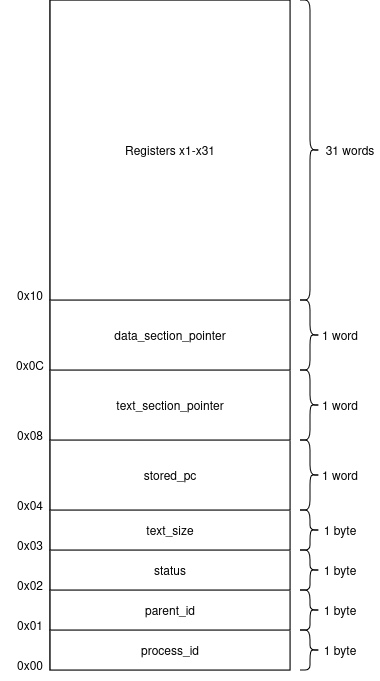
\includegraphics[height=0.6\textheight]{figures/process_structure.png}
    \centering
    \caption[Process Structure]{This figure shows the structure of process data stored, with the relative offset for each element and the size of each section}
    \label{fig:proc_struc}
\end{figure}
Due to the limited memory available on the Hifive1, the data required to store information on each process has to be structured carefully, else the memory required to store process information would begin to memory available to the processes themselves. In the current implementation, 35 words are used to store process information.
\\
One byte each is allocated for a process id, process parent id, process status, and size of a processes text section. For process id and process parent id, only one byte is needed as the Hifive1 does not have the memory to support a large of processes, so a theoretical cap of 256 processes is acceptable. Process status can only take 4 values, so only 2 bits of the byte are used, and the text size byte stores the size as a power of 2, where a process has \(2^n\) words, where \(n\) is the value stored. The minimum number of bits needed to store these is 13, however this would need to be padded to either 32 bits, to ensure that the structure remained word aligned, as an attempt to use the load word instruction on a non word aligned address causes a load address misaligned error. Instead each entry is stored as a byte, as this is the smallest size load that RISC-V allows, which avoids the need to use bit masks to retrieve these entries.
\\
One word each is allocated for the processes program counter, text section pointer and address space pointer. Since memory addresses are word length, these cannot be reduced.
\\
The vast majority of the process structure is used storing the 31 general purpose registers. This is required to retain the state of each process in between scheduling. The only option to reduce this would be to limit the amount of registers available to use. Only 31 must be stored as the x0 register is hardwired to zero.
\\
In other systems, information like the processes stack pointer may be stored, however standard RISC-V calling convention specifies x2 to be used as the stack pointer, so separate storing of this information is not required, and allows a process to handle its address space on its own, however on process creation x2 and x3 are initialized as the stack pointer and the global pointer, where the stack pointer points to the bottom of the process address space and the global pointer at the top. This is done to reduce the overhead of processes that use the standard calling convention.
\subsection{States}
\begin{figure}[H]
    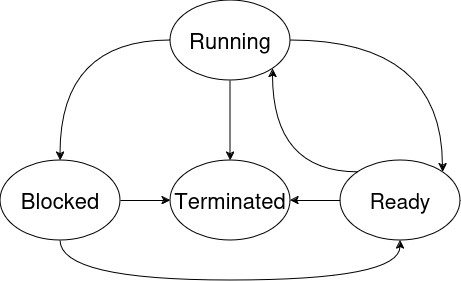
\includegraphics[width=0.8\columnwidth]{figures/states.png}
    \centering
    \caption[State Diagram]{State machine showing the four states a process may be in, and the possible transitions}
\end{figure}
Each process has a state, which indicates how the process should be scheduled. In our model, there are four states that a process can be in; ready, running, blocked, and terminated. Running indicates that the process is currently being executed. A running process can transition to ready if the scheduler preempts the process, or if the process yields to the processor with an environment call. A process will transition to blocked when it makes an interrupt driven \ac{io} call. The blocked process may then transition to ready when the interrupt has been handled. The transition between ready and running is handled by the scheduler, whereas the status of blocked processes are dealt with by each \ac{io} handler. The state value stored in each process entry is used as metadata only except for the terminated state, as instead the scheduler and each \ac{io} handler tracks state by how each process is stored, for instance any process in a queue to be ran is in the ready state, the current process is in the running state, and any processes not in the queue and not running must be blocked. The terminated state indicates to the scheduler that the process should not be re-queued.

\section{Board Boot and Configuration}
On power on the Hifive1 will begin execution at the reset vector of 0x1004, which in this implementation is not configurable and will jump to the Mask ROM at 0x1\_0000, in which similarly cannot be configured in the Hifive1's implementation of the E31, which is the general architecture that the Hifive1's chips is implemented from. The mask ROM will immediately jump to the \ac{otp} memory. This is configurable, but will not be done in this project. This is because the \ac{otp} memory can only be edited by code executing on the board, and only one bit at a time. Since the \ac{otp} memory is executed as part of the boot sequence, if it is programmed in a way that does not jump to code in flash or memory it will prevent the board from executing code, which also means that the malfunctioning \ac{otp} code cannot be fixed, leaving the board in an unrecoverable state. This danger is obviously unacceptable for this project, so the \ac{otp} memory will be left to its default, which will jump to 0x2000\_0000, which is the beginning of flash memory.\\
From that point, execution of the system setup begins.
On the Hifive1, there are several important configuration options that affect general operation of the board. The most notable of these are the clock settings, as these indicate the frequency of the processor, input and output frequencies, and timer interrupts. This is the second thing configured during boot, after zeroing the registers.
\begin{enumerate}
    \item The pc is set to 0x2000\_0000
    \item The system stack pointer and global pointer is set, and the other registers are zeroed
    \item Both high frequency and low frequency clocks are set to 16 MHz and ~32 KHz
    \item The trap vector base and mode is set
    \item The GPIO is set to enable the LEDs and the UART
    \item The UART is configured, and the UART print queue is created
    \item The external interrupt settings are configured
    \item The scheduler queue and available process stack are created
    \item The process table is populated with basic information including each processes address space, and each process is added to the available process stack
    \item Any initial user applications are added to the queue for scheduling
    \item The scheduler is started
\end{enumerate}

\subsection{Clock settings}
The Hifive1 has 3 clock regions, a high frequency clock, a low frequency clock, and a clock used to drive the JTAG connection. The JTAG driver is constant and only used for debugging through JTAG, so is not relevant here.
\\

\begin{figure}[H]
    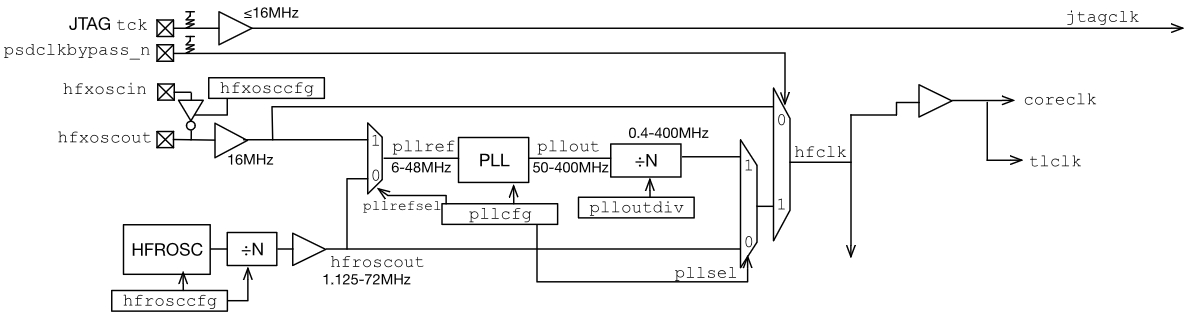
\includegraphics[width=0.9\columnwidth]{figures/hfclock.png}
    \centering
    \caption[High Frequency Clock Diagram]{The high frequency clock generation scheme, specifying how the high frequency clock is driven and configured, taken from the Sifive FE310-G002 Manual\cite{sifive_manual}}
\end{figure}
The high frequency clock controls the processor frequency, and the baud rate of input and output is derived from it. The high frequency clock can be driven from two sources, an internally trimmable high frequency ring oscillator and an external high frequency crystal oscillator. The ring oscillator can produce frequencies ranging form ~1 MHz to 75 MHz, whereas the crystal will produce a constant frequency of 16 MHz. Both of these clock sources may be used `as is', or can be modified using a PLL and divider, giving a available range of 48 MHz to ~400 MHz. 
\\
\begin{figure}[H]
    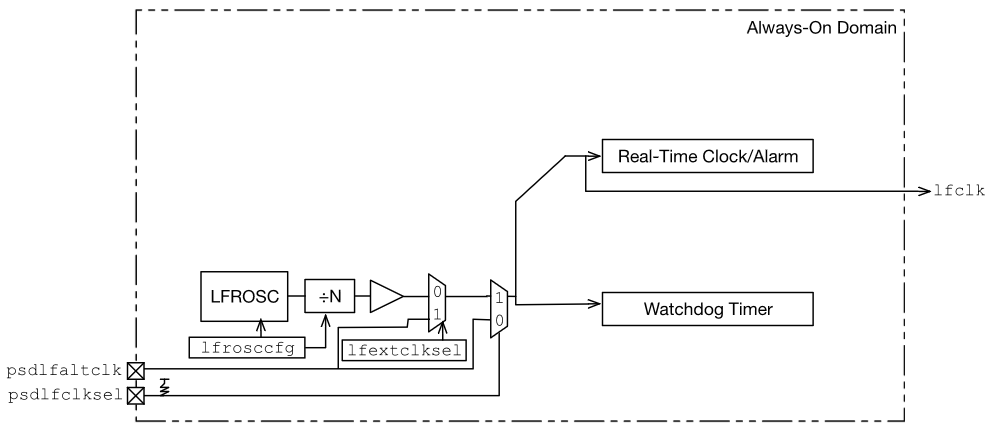
\includegraphics[width=0.9\columnwidth]{figures/lfclock.png}
    \centering
    \caption[Low Frequency Clock Diagram]{The low frequency clock generation scheme, specifying how the low frequency clock is driven and configured, taken from the Sifive FE310-G002 Manual\cite{sifive_manual}}
\end{figure}
The low frequency clock is part of the Hifive1 `always on block' and controls the watchdog timer, which can be used to cause a reset on malfunction, and both the real-time clock and the machine timer, both of which are used to generate timed interrupts. Similar to the high frequency clock can be driven from a ring oscillator or from an external clock, which in the Hifive1 is a crystal oscillator. The low frequency ring oscillator functions at 1.5 kHz to 230 kHz using a frequency divider, and the implemented external clock runs at a constant 32.768 kHz, with no option to divide the frequency.
\\
For both clock domains, the crystal oscillator was chosen. The ring oscillator gives the option to operate at a higher frequency, which would result in a higher number of operations per second. While in a practical operating system this would be desirable, since this system is not intended for practical use, a constant frequency was more desirable as it would give more predictable results, and makes \ac{io} operations more reliable. For the low frequency clock, a high frequency would be beneficial for a real time system as the higher frequency would allow for more precise timing of interrupts and other functions, however for an interactive system this precision is not required, and so similar to the high frequency domain the constant frequency of a crystal oscillator was selected.
% Add in trap implementation not theory
% move this to background
\section{Traps}
\subsection{Configuration}
When an enabled trap is raised, the pc is set to the trap vector according to the trap mode. The trap vector and mode are stored in the 32 bit csr \textit{mtvec}. In this csr, bits [1:0] are used to store the mode, where 0 is direct mode and 1 is vectored mode. Bits [31:2] represent vector base address, which is the top 30 bits of a 32 bit address. Since this is stored as 30 bits, two zeros are added to pad the value. This means that the trap handler address must be aligned to 64 bytes, which can be done simply using the .align pseudo-instruction. When in direct mode, a trap will set the pc to the base vector address, whereas in vectored mode only synchronous traps are set to the base address, and asynchronous traps set the pc to the base address added to four times the trap code. For this system the vectored mode was chosen. This was because the asynchronous traps are more frequent than synchronous traps, and by jumping to the specific trap call directly a large amount of overhead is skipped. This is relevant for functions like the preemptive scheduler, as it reduces the time to switch processes, which will allow the preempter to be more effective with short quantum's.
\subsection{Asynchronous Traps}
Due the use of vectored trap mode, instead of having one single handler for asynchronous traps, each interrupt has it's own handler. Since the Hifive1 does not implement a supervisor mode, there are only 3 available interrupt types, software, timer and external. The software interrupts are not used, as they are mainly used for communication between processes running in parallel, and the Hifive1 only has a single core, so this can be reserved for another use. The machine timer is used for the preemptive scheduler, which will be explored in detail in further sections. Finally the external interrupts, the handler will read from the \ac{clint} claim/complete register. This will provide the handler with the highest priority interrupt code, which will then be used in a jump table to execute the correct interrupt, and once completed the same value is written back to the claim/complete register to indicate that the interrupt has been handled. The interrupts implemented in this will be explored in further sections.
\subsection{Synchronous Traps}
The trap code for synchronous traps can be fetched from the \textit{mcause} register. This can then be used with a jump table to handle the correct trap. Synchronous traps fall into two main categories; environment calls and exceptions. For exceptions, most function by outputting an error message, and then depending on the severity of the exception either halting execution or returning execution to the cause in the case of a non fatal error.
\subsubsection{Environment Calls}
Environment calls function using the standard calling convention, where the value in a7 is used to determine the desired environment call, and a0-6 are used as arguments like a standard function. Since the board implements user mode and machine mode, there are two separate codes for environment calls from user mode and machine mode however for most cases these can be combined.
\section{Scheduler}
This system will be implemented with an interactive scheduler. The functions that the scheduler must perform are storing all the processes that are in the ready state, running ready processes, and preempting processes that have been running for longer than the quantum, which is the amount of time given to the process. The scheduler will be ran mainly through the use of interrupts.
\subsection{Creating a Process}
On boot, a table of process entries is allocated in memory, and parts of each are initialized, such as each processes address space and their stack and global pointers. The scheduler will then store the pointer to each entry on a stack, which is used to distribute a process entry to each new process. When a new process is created, the pointer on the top of the stack is used to populate that entry with information about the new process, including the start of the text section which is also used as the processes initial pc, the size of the text section, and the process is also given a sequentially generated process id. Once the process is initialized, it is then added to a queue in the scheduler, which is implemented as a circular queue.
% grammar here!!
\subsection{Running a process}
To make a process run, the scheduler will first dequeue from the ready processes queue. This will then be used to set the processes state. The stored pc will be used to set the \textit{mepc} csr, which stores the value of the pc to return to when mret is called, as the mret instruction restores the previous privilege mode and sets the pc to the value in \textit{mepc}. The \ac{pmp} is then set to allow access to that processes' address space, as well as allowing read access to that process text section in the Flash memory. The state of the process in the process entry is changed to running. Then most of the registers have their values set, except for t1-4. This is because before these values are set, the scheduler sets the quantum for the process by setting the timer comparison to the current time plus the quantum, and this requires a minimum of 4 registers to do. This is done as close to the start of execution instead of before the registers have their state set, as this ensures the time allowed for each process is as close to the specified quantum as possible. Finally the last 4 registers are set and MRET is called, which begins the execution of the process. The process will then execute until it is stopped, which can happen in five different ways. The first three is where execution is handed back to the scheduler, through either yielding, termination, blocking, or preemption. The final way is that a process could cause an error which could either halt execution, return control to the application or cause it to be terminated.
% grammar here aswell!
\subsection{Preemption and Scheduling}
If either a yield or a termination occurred control will return to the scheduler without preemption. Each process is given a 50 millisecond quantum, after which it is preempted and control is given to the scheduler. This time includes execution of user code as well as environment calls, however a process cannot be preempted in the middle of an environment call, so if a process reaches the end of its execution time during an environment call, it will be preempted as soon as the system returns to the user code. As previously mentioned, the preemption is timed using the machine timer interrupts. The machine timer was chosen over the timer interrupt generated by the AON unit, as the latter interrupt is part of the external interrupts so there is an increased amount of overhead required for it to be processed. Using the machine timer interrupt also addresses another problem, which is maintaining the state of the process. When the preemption occurs, the first thing that must happen is that the processes registers must be saved to the process entry, which requires the global pointer. The global pointer is a constant value, as it always points to top of the machine address space, however to use it, it must be stored into a register, which requires that registers value to be store to the machine stack. For this we use the \textit{mscratch} csr to store the machine pointer during normal execution, which when in machine mode we swap with the current processes stack pointer. This allows us to use the machine stack while also storing the processes stack. In addition to the global pointer we also save the value in t0 and t1 to store the process entry pointer, and to pop and store the values back from the stack and the \textit{mscratch} csr, before saving each of the remaining 26 registers. The operations of the preempter occur as follows:
\begin{enumerate}
    \item The \ac{pmp} is reset, clearing all user memory access
    \item The fence.i instruction is called, which invalidates all entries in the instruction cache
    \item The process sp is switched with the machine sp in the \textit{mscratch} csr
    \item Registers gp, t0, and t1 are pushed to the stack
    \item The global pointer is loaded into gp, and used to load the current process entry pointer into t0
    \item The 3 values pushed to the stack are each pop into t1 and then stored into the process entry, as well the the value that was swapped into the \textit{mscratch} csr
    \item All 26 remaining registers are stored to the process entry
    \item The value stored in the \textit{mepc} csr is loaded and stored
    \item If the process had the running state, it is changed to ready, otherwise it remains unchanged.
    \item If the status is terminated, add the process entry pointer to the free entry stack
    \item Else add the pointer to the process queue
\end{enumerate}
\subsubsection{Blocking and Yielding}
Scheduling ready processes and terminated processes is intuitive, however when a process is blocked, the scheduler is instructed to ignore that process. This is because it is the job of the blocking source to store its blocked processes. This reduces the complexity of the scheduler and gives more freedom as to how a process in unblocked. \\
When a process is yields or is blocked, the scheduler is requested to schedule a new process. One method of doing this would be to call the scheduler directly from whatever environment call or interrupt caused the yield or block. However this could create an inconsistent state, as the scheduler preempter is always called from an interrupt to user code. Because of this, when a process yields or is blocked, it simply zeros the timer compare, so that when it returns to the user code it will immediately raise an exception, allowing the scheduler to handle the process as normal.
\section{Memory Management}
\subsection{Address Spaces}
\begin{figure}[H]
    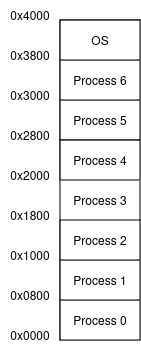
\includegraphics[height=0.3\textheight]{figures/dtim.png}
    \centering
    \caption[Layout of memory]{The sections of the DTIM serving as memory, with the address offsets from 0x80000000}
\end{figure}
For this project, RISC-V's \ac{pmp} was used to implement and enforce address spaces. The Hifive1 has two forms of memory, a 512 MiB flash memory to serve as ROM and an 16 KiB L1 \ac{dtim} which served as RAM. Both of these sections allow for execution of code. Because of this and the limited amount of RAM, the text section of each program will be stored on and executed from the flash memory. The 16KiB of RAM is split into 8 address spaces, making each space 2KiB. This size was chosen as a balance between number of available processes and amount of memory available to each process, as well as ensuring that the space needed to store information of the processes did not take up the majority of the machine address space. This is because since each process entry requires 35 words or 140 bytes, so if split into 8 address spaces there will be 7 available processes, which would take 980 bytes. So with only 7 processes, the process entry table would already take ~48\% of the machine address space. This could be adjusted by keeping the machine address space at 2KiB while decreasing the address space size to each process, however it is useful to have the address spaces be in powers of 2, as will be discussed later with the \ac{pmp}. If equal sized spaces were maintained but split into 16 1 KiB spaces, the 15 process entries would need 2100 bytes, which is over 200\% of what is available. If we were to increase the size of the spaces to 4 KiB, that would only make 4 address spaces, with only 3 available processes, which is too small to be practical.
\subsection{Address Space Layout}
\begin{figure}[H]
    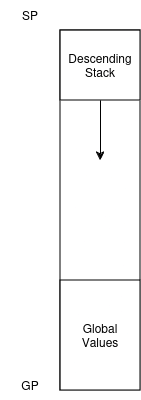
\includegraphics[height=0.3\textheight]{figures/addr_space.png}
    \centering
    \caption[Process Address Space]{The structure of each of the seven process address spaces, featuring the stack and globals}
\end{figure}
Each 2 KiB address space has 2 pointers. The global pointer, gp, points to the bottom of the address space, and is used to store global variables for a process, so should not change unless a program chooses to use the gp register for another purpose. The stack pointer, sp, initially points to the word above the top of the address space. This is used to implement a full descending stack. Sp will always store the pointer to the last item added to the stack, so when the stack is empty it will point to the word outside of the stack.
\subsection{PMP Use}
To enforce the address spaces, RISC-V's PMP is used. PMP allows us to specify sections of code to have have restricted access to calls from user mode. This is done by setting the values in the \textit{pmpaddr} and \textit{pmpcfg} CSRs. It can be done in two ways, either the top of range setting which protects the region between a specified top address and either the previously referenced address, or 0x00000000. This allows a precise range however it would require storing two values in each process for its text section. The other method is to specify an address which is naturally aligned to a power of two. This means that the address is a multiple of that power of two. The value of the power of two is specified by using the trailing zero bits of the naturally aligned address, where all but the most significant zero bit is set to one. The configuration for each is stored as one byte, with 5 fields, R, W, X, A, and L. R, X, and W control the read, write and execution access in each region, A controls whether that control region is active and the method which the region is specified, and L will lock the settings and also enforce the settings to both user mode and machine mode until reset. When L is not set, code executed in machine mode will ignore the \ac{pmp} settings.\\
These addresses are stored in the CSRs \textit{pmpaddr0} to \textit{pmpaddr7}, which means that the Hifive1 implements up to 8 PMP controlled regions. The configuration of each of these addresses is stored in the CSRs \textit{pmpcfg0} and \textit{pmpcfg1}, which each control \textit{pmpaddr0-3} and \textit{pmpaddr4-7}, respectively.\\

Since the address spaces in RAM are constant the pmpaddr value can be generated by setting address[8] low and address[7:0] high. The text section of a process has a variable size, which is stored as the value \(n\), where the size of the section is \(2^n\) words. There are then two cases to consider when implementing this. When \(n == 0\) it represents the case when the size of the section is only one word. Since this will always result in a naturally aligned address, there is a separate value of A to represent this NA4 case, so all that is required for this case is to set A to 2, and specify the word address. The general case where \(n > 0\) works as previously specified. 
\section{IO}
The Hifive1 has few forms of IO available. Most forms of IO are driven through the \ac{gpio}. This controls the function of each of the Arduino-compatible pins, as well as up to two alternate functions for each GPIO pin, which is used to control the \ac{uart}, \ac{spi}, and \ac{pwm}, as well as three LED's featured on the board. 
\subsection{LEDs}
The simplest form of \ac{io} on the Hifive1 are the three LED's, which can be used as simple indicators, however they utilize the \ac{gpio} just as the other \ac{io} functions do. The green, red, and blue LED's use GPIO pins 19, 21, and 22 respectively. To use them, the bits 19, 21, and 22 in the GPIO output enable register, memory mapped to 0x1001\_2008, must be set low, since the GPIO uses low enable. This enables the LED's to function, which can turned on and off by setting the bits in the GPIO output register similarly to how they were set for the enable register.
\subsection{Text input and output}
The main way a user may interact with a program in this system will be through the use of a terminal, which requires the need to print and receive text. To do this, we will utilize one of the two \ac{uart} peripherals. This will allow us to send and receive text from a host machine that is connected via the USB port.
\subsubsection{Host machine}
When the Hifive1 is connected to a host machine, the two UART peripherals are represented as two ttyACM devices, which can be interfaced with using the two files /dev/ttyACM0 and /dev/ttyACM1. To fetch and send data, the terminal used must be configured to function at the target baud rate.
\subsubsection{UART configuration}
To enable the use of \ac{uart}, the specific peripheral must be enabled through the \ac{gpio}. To do, bits 16 and 17 of the iof\_en register must be set to 1, and same bits of iof\_sel should be set to 0. This toggles GPIO\_16 and GPIO\_17 from software control to hardware control from the UART0 peripheral. After this, UART0 must be configured. The first setting to alter is the frequency divider, which is used to determine the baud rate of the peripheral from the high frequency clock. This uses the formula \[f_{baud}=\frac{f_{hfclk}}{div+1}\]. The target baud rate will be 115200 Hz. Using the hfclock frequency of 16~MHz, we can deduce that the required divisor will be 138, which give us the actual baud rate of 115107 Hz, which has an error 0.08\%. Other settings include setting the rx\_en and tx\_en to high, to enable both reading and transmitting. Other configurations include the watermark level, which will be discussed in a later section.
\subsubsection{Transmitting}
The transmission of data from user is interrupt driven. To begin a transaction, a process will make a environment call, passing it a pointer to the first character of a zero terminated string as an argument. First the calling process is blocked, and that process is queued onto a queue structure, which stores all processes that are currently blocked due to an ongoing request to transmit. The string pointer is then queued onto a second queue, with all the processes strings. It then checks if the transmission interrupts are already enabled due to other requests, and enables them if not, before returning from the environment call. The transmission interrupts function of the watermark value defined in tx\_en in combination with the transmission queue. The UART has a queue that stores up to eight bytes during transmission. By setting the transmission watermark to one, it will raise an interrupt whenever the the queue has less than one element in it. When this is enabled, the initial interrupt can be used to add to this queue until it is full, and then return to the calling environment. The UART will then transmit this data, and once the queue is empty again, another interrupt will be raised and the queue will be filled again. This will continue until the end of the string is reached, at which point the interrupt will dequeue from the blocked process queue and unblock that process. It will then determine if there is another string to print, which if there is it will repeat the same process, and if there is not it will disable the transmission interrupts.
\subsubsection{Receiving}
Unlike the transmission, receiving is done using programmable \ac{io}. This is done because only one stream of serial \ac{io} is available, because although there are two UART units on the board, UART1 is reserved for use by the wireless module, so only UART0 is available for general use. If the input was interrupt based, it would mean it would allow an output to interrupt a users command line while they were typing. This could be avoided by using a more complex interaction system, or by developing a more complex terminal program on the host computer. Because of this, when a process asks to receive information, it makes an environment call which takes a pointer to a buffer in memory as an argument, and will receive characters from UART0 until it receives a zero byte, at which point control is return from the environment. In future this should also be done in a similar method to transmission.

% Testing and evaluation is very well thought through and described. The report could be used to reproduce the work.
\chapter[Evaluation]{Evaluation}
\label{cha:eval}
In this section, I will discuss the capabilities of the designed operating system with comparisons to the original concepts it was implementing to evaluate its effectiveness and completeness.
\section{Challenges}
Since this project is hardware based, there are several complications when it comes to testing that do not occur in standard software. This is because the tools available to validate programs are less available, which results on a far greater reliance on manual checking as opposed to automated testing. This problem is made worse as many of the methods of checking for correct execution are reliant on standard IO, which is not available to us as the IO itself is being developed.\\
Another challenge is the problem of developing with interrupts that are triggered by uncontrollable events, or events that need to function at a high frequency. These include timer interrupts, and external interrupts that function asynchronously like the UART. These limit the functionality of breakpoints, as often the asynchronous behaviour can continue while execution of the rest of the processor is paused, which puts the system into a state that would not occur during normal execution.
\section{Dissasembly}% find better section title
The first step to ensuring code is correct was to ensure that the assembled code was assembled and linked correctly. To facilitate this, on assembly the makefile was configured to dissasemble the generated executable, using objdump from the riscv-gnu-toolchain. This enabled me to ensure that the structure of each section was maintained, which is important as many parts of the system require memory alignment, for example in the jump tables used in the enviroment handler and the exception handler require the branch instructions to be word aligned, and that the spacing between entries is correct. The decompilation was also vital when developing the toolchain, as it allowed me to validate that the system would be loaded correctly between Flash and the DTIM.
\section{Breakpoints and Inspection}
Of the tools available to debug, one of the most powerful tools is the JTAG interface. The JTAG interface allows an external connection to access the debug CSRs of the system, which allows a host machine to control the execution and memory state of the board, through the use of breakpoints and step through execution and memory commands. To utilise this, I used GDB to load code onto the board, at which point GDB could interface via JTAG to create a similar debug enviroment on the host machine to the debug enviroment of a standard program. 
% \section{Design Reflections}
% memory man: was the constant address space sufficient, or should another system have been implemented, like a dynamic system that include requests for heap memory, instead of providing a constant amount
% processes: was the project developed to allow for sufficient interprocess communication? programs could create forks and new processes however no design was included to allow for these to communicate after the initial creation
% Lack of method to write and user code seperately to the oa
% Limited IO, could more IO been developed to make the system more interactive, for instance use of the aduino compatable pins, or basic use of the wireless chip.
% Implemented IO, was all the functions built to function? Inputs blocked execution, was this appropriate or could a better design be made to allow this to be interrupt based
% Was the choice of interactive shceduler correct? or should of a batch system have been chosen due to the limited io of the device limiting the interactivity of the device
% Did the os function? at what rate did it execute? how did the quantum affect the interactivity
\chapter[Evaluation]{Evaluation}
\label{cha:eval}

\bibliography{refs}             % this causes the references to be
                                % listed

\bibliographystyle{abbrv}       % this determines the style in which
                                % the references are printed, other
                                % possible values are plain and abbrv
%% Appendices start here
\appendix
\include{appendix1}
\end{document}
